%\section{Tabelas}\label{tabelas}
\onecolumn

\section{Figuras}\label{figs}

\subsection{Valgrind}\label{val}

\begin{figure}[h]
	\centering
	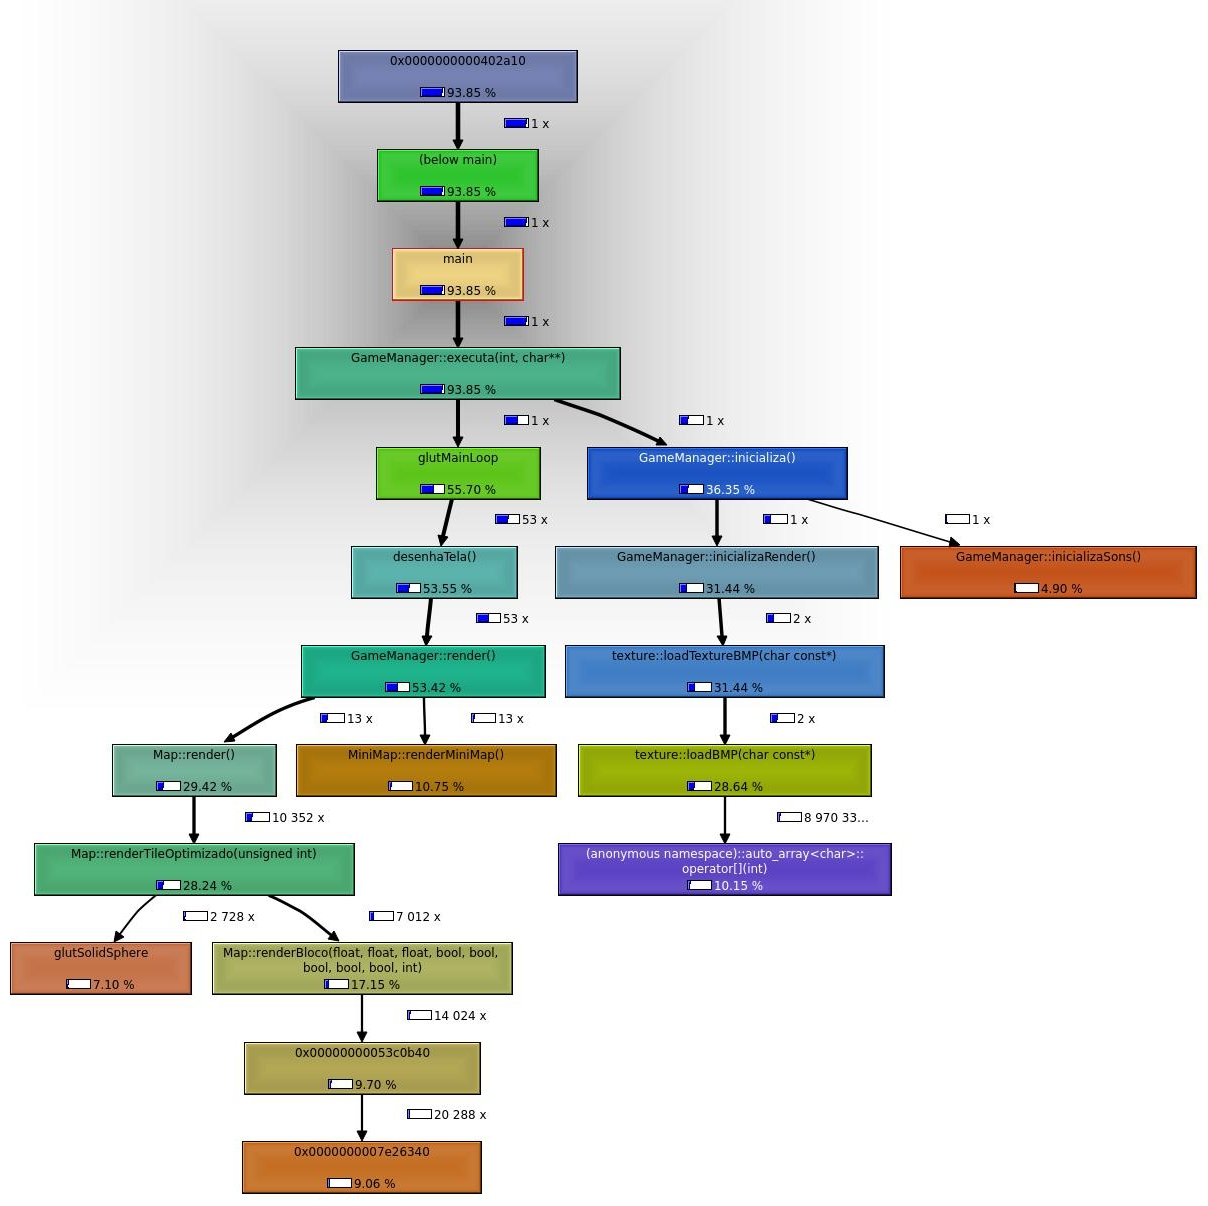
\includegraphics [scale=0.5,angle=0,keepaspectratio=true]{./fts/callgrind/img3}
	\caption{Saída gerada pelo Valgrind}
	\label{valgrind}
\end{figure}

\newpage
\subsection{Diagrama de Classes}\label{class}
\begin{figure}[h]
	\centering
	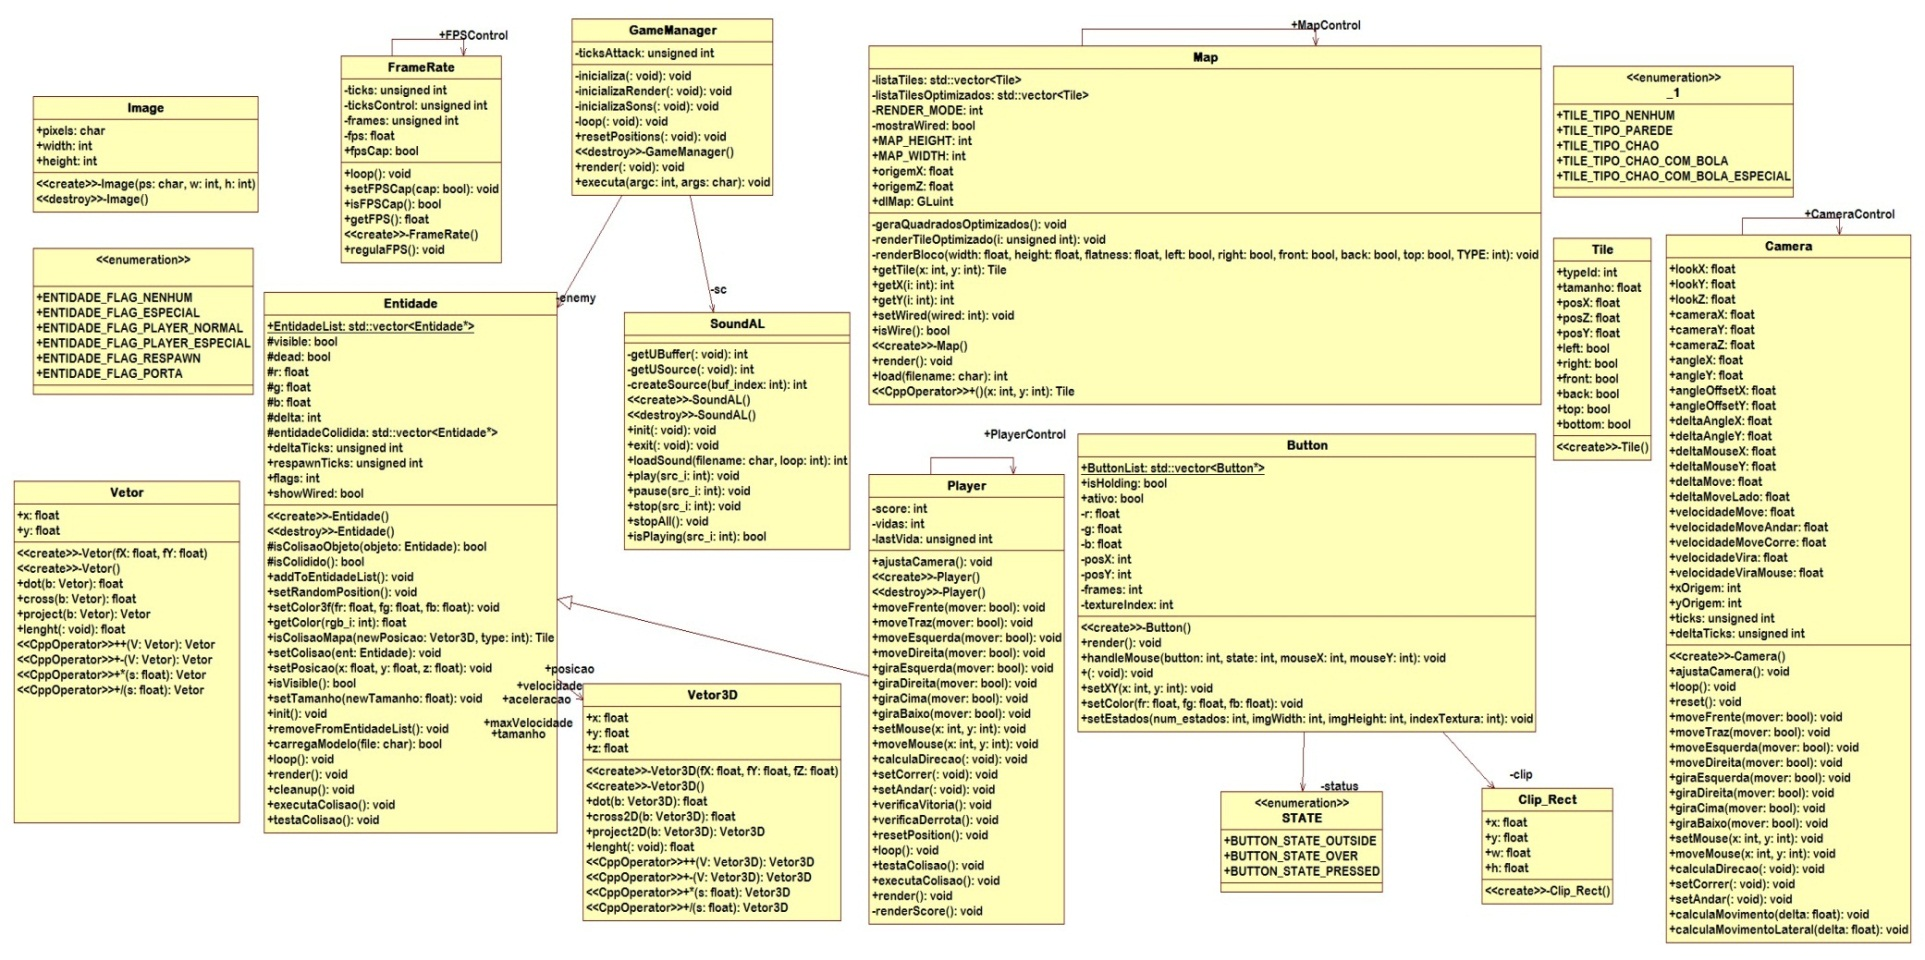
\includegraphics [scale=0.92,angle=90,keepaspectratio=true]{./fts/diag_class}
	\caption{Diagrama de classes}
	\label{classes}
\end{figure}

\newpage
\section{Códigos Fontes}\label{src}

%------------------------------------------------------------------------------%		
% Anexar source main.c com link
%\hypertarget{main}{
%\lstinputlisting[language=C,texcl=true]{../main.c} }
%anexar source main.c sem link
%\lstinputlisting[language=C]{../main.c}
%------------------------------------------------------------------------------%		
%\cite{ti_exemplos}
%\tableofcontents %Índice de conteúdos
%\listoftables %Lista de tabelas
%\listoffigures %Lista de figuras
%------------------------------------------------------------------------------%		
\subsection{Headers}\label{.h}

\subsubsection{Button}
\lstinputlisting[language=C++]{../../trunk/button.h}
\subsubsection{Camera}
\lstinputlisting[language=C++]{../../trunk/camera.h}
\subsubsection{Defines}
\lstinputlisting[language=C++]{../../trunk/defines.h}
\subsubsection{Entidade}
\lstinputlisting[language=C++]{../../trunk/entidade.h}
\subsubsection{Eventos}
\lstinputlisting[language=C++]{../../trunk/eventos.h}
\subsubsection{Framerate}
\lstinputlisting[language=C++]{../../trunk/framerate.h}
\subsubsection{Game Maneger}
\lstinputlisting[language=C++]{../../trunk/gamemanager.h}
\subsubsection{Map}
\lstinputlisting[language=C++]{../../trunk/map.h}
\subsubsection{Minimap}
\lstinputlisting[language=C++]{../../trunk/minimap.h}
\subsubsection{Modelo de objetos}
\lstinputlisting[language=C++]{../../trunk/model_obj.h}
\subsubsection{Player}
\lstinputlisting[language=C++]{../../trunk/player.h}
\subsubsection{Sound}
\lstinputlisting[language=C++]{../../trunk/soundAL.h}
\subsubsection{Texto}
\lstinputlisting[language=C++]{../../trunk/text.h}
\subsubsection{Carregamento de textura}
\lstinputlisting[language=C++]{../../trunk/textureloader.h}
\subsubsection{Tile}
\lstinputlisting[language=C++]{../../trunk/tile.h}
\subsubsection{Vetor 3D}
\lstinputlisting[language=C++]{../../trunk/vetor3d.h}
\subsubsection{Vetor}
\lstinputlisting[language=C++]{../../trunk/vetor.h}

\subsection{Sources}\label{.cpp}

\subsubsection{Button}
\lstinputlisting[language=C++]{../../trunk/button.cpp}
\subsubsection{Camera}
\lstinputlisting[language=C++]{../../trunk/camera.cpp}
\subsubsection{Defines}
\lstinputlisting[language=C++]{../../trunk/defines.cpp}
\subsubsection{Entidade}
\lstinputlisting[language=C++]{../../trunk/entidade.cpp}
\subsubsection{Eventos}
\lstinputlisting[language=C++]{../../trunk/eventos.cpp}
\subsubsection{Framerate}
\lstinputlisting[language=C++]{../../trunk/framerate.cpp}
\subsubsection{Game Maneger}
\lstinputlisting[language=C++]{../../trunk/gamemanager.cpp}
\subsubsection{Map}
\lstinputlisting[language=C++]{../../trunk/map.cpp}
\subsubsection{Minimap}
\lstinputlisting[language=C++]{../../trunk/minimap.cpp}
\subsubsection{Modelo de objetos}
\lstinputlisting[language=C++]{../../trunk/model_obj.cpp}
\subsubsection{Player}
\lstinputlisting[language=C++]{../../trunk/player.cpp}
\subsubsection{Sound}
\lstinputlisting[language=C++]{../../trunk/soundAL.cpp}
\subsubsection{Texto}
\lstinputlisting[language=C++]{../../trunk/text.cpp}
\subsubsection{Carregamento de textura}
\lstinputlisting[language=C++]{../../trunk/textureloader.cpp}
\subsubsection{Tile}
\lstinputlisting[language=C++]{../../trunk/tile.cpp}



\subsubsection{Makefile}
\lstinputlisting[language=make]{../../trunk/Makefile}
\subsubsection{README}\label{README}
\lstinputlisting[language=make,texcl=true,numbers=none]{../../trunk/README}

%



%-------------------------------------------------------------------------

% End of code
% End of code


%Inclusão de Figuras
%--------------------Figura logo da UnB----------------------------------------%
%\begin{figure}[h]
%	\centering
%	\includegraphics [scale=1,angle=0,keepaspectratio=true]{./fts/unb}
%	\caption{Logo da UnB}
%	\label{unb}
%\end{figure}
%--------------------Figura logo da UnB----------------------------------------%
%\begin{SCfigure}[1][h] %%Cuidado..ela não se mantem no lugar
%  \centering
%  \includegraphics[width=4cm]{./fts/unb}
%  \caption{Logo da UnB.}
%  \label{unb1}
%\end{SCfigure}


%\begin{multicols}{4}
%\tikzstyle{cloud} = [draw, ellipse,fill=red!20, node distance=3cm,
%    minimum height=2em]
%\tikzstyle{phanton} = []   
%\tikzstyle{line} = [->,bend left] %[draw, -latex']
%\tikzstyle{arrow} = [loop above]
%
%\begin{center}
%\begin{tikzpicture}[node distance = 2cm]
%	\tiny\ttfamily
%	%-- Estados
%	\node [cloud] (E0) at(0,2) {E0};
%	\node [cloud] (E1) at(2,1) {E1};
%	\node [cloud] (E2) at(2,-1) {E2};
%	\node [cloud] (E3) at(0,-2) {E3};
%	\node [cloud] (E4) at(-2,-1) {E4};
%	\node [cloud] (E5) at(-2,1) {E5};
%	%-- setas
%	\path (E0) edge [line] (E1);
%	\path (E1) edge [line] (E2);
%	\path (E2) edge [line] (E3);
%	\path (E3) edge [line] (E4);
%	\path (E4) edge [line] (E5);
%	\path (E5) edge [line] (E0);
%	%-- Desvios
%	\path (E0) edge [draw,loop above] node{controle1=1} (E0);
%	\path (E3) edge [draw,loop below] node{controle2=1} (E3);
%	\path (E2) edge [bend right,->]  node[anchor=east]{controle1=1\&\&controle2=0} (E0);
%	\path (E5) edge [bend right,->]  node[anchor=west]{controle1=0\&\&controle2=1} (E3);
%\end{tikzpicture}
%\\\hypertarget{diagrama}{Diagrama de Estados}
%\end{center}


%\end{multicols}


%\setcounter{diagheight}{50}
%\begin{chart}
%\reqfullcourse 50,45:{ }{GameManager::Loop}{gamemanager.cpp}
%\reqhalfcourse 30,30:{2813}{Loop()}{MWF 8:30}
%  \prereq 50,45,30,30:
%
%\reqhalfcourse 20,20:{2813}{testColisao()}{MWF 8:30}
%  \prereq 30,30,20,20:
%\end{chart}

% Define block styles
\tikzstyle{decision} = [diamond, draw, fill=blue!20, 
    text width=4.5em, text badly centered, node distance=3cm, inner sep=0pt]
\tikzstyle{block} = [rectangle, draw, fill=blue!20, 
    text width=5em, text centered, rounded corners, minimum height=4em]
\tikzstyle{line} = [draw, -latex']
\tikzstyle{cloud} = [draw, ellipse,fill=red!20, node distance=3cm,
    minimum height=2em]

%\begin{figure}
%    \centering
%\begin{tikzpicture}[node distance = 2cm, auto]
%	
%	\node [block] (init) {Manager\\executa()};
%	
%\end{tikzpicture}
%\caption{Diagrama de Fluxo}
%\end{figure}

%-------------------------------------------------------------------------------

%\begin{figure}
%    \centering
%\begin{tikzpicture}[node distance = 2cm, auto]
%    % Place nodes
%    \node [block] (init) {initialize model};
%    \node [cloud, left of=init] (expert) {expert};
%    \node [cloud, right of=init] (system) {system};
%    \node [block, below of=init] (identify) {identify candidate models};
%    \node [block, below of=identify] (evaluate) {evaluate candidate models};
%    \node [block, left of=evaluate, node distance=3cm] (update) {update model};
%    \node [decision, below of=evaluate] (decide) {is best candidate better?};
%    \node [block, below of=decide, node distance=3cm] (stop) {stop};
%    % Draw edges
%    \path [line] (init) -- (identify);
%    \path [line] (identify) -- (evaluate);
%    \path [line] (evaluate) -- (decide);
%    \path [line] (decide) -| node [near start] {yes} (update);
%    \path [line] (update) |- (identify);
%    \path [line] (decide) -- node {no}(stop);
%    \path [line,dashed] (expert) -- (init);
%    \path [line,dashed] (system) -- (init);
%    \path [line,dashed] (system) |- (evaluate);
%\end{tikzpicture}
%\caption{Diagrama de Fluxo}
%\end{figure}
